\documentclass[final,5p,times,twocolumn,authoryear]{elsarticle}
\usepackage{lineno,hyperref}

\journal{Journal of Urban Management}
%\journal{}

\begin{document}

\begin{frontmatter}

\title{Trade-offs between sustainable development goals in systems of cities}

%\author{}
\author[label1,label2,label3]{Juste Raimbault\corref{cor1}}
\author[label4]{Denise Pumain}

\address[label1]{LASTIG, Univ Gustave Eiffel, IGN-ENSG}
\address[label2]{CASA, University College London}
\address[label3]{UPS CNRS 3611 ISC-PIF}
\address[label4]{UMR CNRS 8504 G{\'e}ographie-cit{\'e}s, Universit{\'e} Paris 1}

\cortext[cor1]{Corresponding author: juste.raimbault@polytechnique.edu}



\begin{abstract}
    
    Sustainable Development Goals are intrinsically competing, and their embedding into urban systems furthermore emphasises such compromises. When observed at the scale of systems of cities, such concern is considered as a series of innovations that challenges the adaptive capacity of urban systems. The spatial complexity, the non-optimal nature of such systems, and the multi-objective aspects of their agents, are among the reasons that raise difficulties when trying to adjust local policies through promoting innovation in order to satisfy at least a couple of SDGs simultaneously. As we lack enough empirical evidence, we propose in this paper to use a stylised simulation model for systems of cities, focused on innovation diffusion and population dynamics, to show how trade-offs may operate at such a scale. We proceed in particular to a bi-objective optimisation of emissions and innovation utilities, and show that no single urban optimum exists, but a diversity of regimes forming a compromise between the two objectives.
\end{abstract}

\begin{keyword}
Sustainable Development Goals; Systems of Cities; Urban Dynamics; Innovation Diffusion
\end{keyword}

\end{frontmatter}

%\end{document}

\linenumbers

\section{Introduction}

\subsection{Urban systems and urban sustainability}

The 17 Sustainable Development Goals that were defined by the United Nations in 2015 \citep{nations2015sustainable} are challenging the adaptation capability of many cities in the world. As they host a growing proportion of the world population and are responsible for a large part of greenhouse gas emissions \citep{christen2014atmospheric}, cities are at the core of environmental transition policies \citep{romero2011cities}. Indeed, cities are explicitly mentioned in SDG 11 \citep{nations2015sustainable}: ``Make cities and human settlements inclusive, safe, resilient, and sustainable''. This citation demonstrates that many other SDGs involving a diversity of urban issues and stakeholders are already embedded in that specific goal \citep{vaidya2020sdg}.

In the ongoing adaptive process of the environmental transition, cities are not isolated. They have been engaged for long in a co-opetition process for attracting population and economic activities that have created many interdependencies in their evolution leading to interpret cities as ``systems within systems of cities'' \citep{berry1964cities}. These systems of cities are an almost universal form of spatial organization of societies to inhabit the earth space. This organization has proven to be very sustainable for several millennia, because it offered a way to continuously adapt the political, economic and technological innovations that societies imagined over the centuries \citep{pumain2020theories}. That remarkable ability to resilience through self-renewal has expanded all over the world up to the point that the largest metropolises may have now become ``global rulers'' \citep{glaeser2020urban}. However, for the last few decades urban systems seem to be threatened by excessive emissions and overexploitation of the planet's energy and material resources \citep{nijkamp2014sustainable,kourtit2020global}. While demographic and economic growth have supported and accelerated the development of urbanization and the proliferation of systems of cities for two centuries, they are now accused of being the cause of climate change problems and the rise of social inequalities \citep{davis2006planet,glaeser2009inequality}. It seems that the excessive mobility associated with the fragmentation of the value chains of globalized production has progressively decoupled urban expansion from the proper management of planetary resources \citep{rozenblat2018urban}. It is unlikely that the technological solutions that are provided under the label of ``smart cities'' could easily solve these problems \citep{caragliu2011smart,kourtit2020global}, especially because of the huge diversity of cities internal layouts and their already established networks operating internal and external interactions \citep{caruso2022no}.


\subsection{Investigating transitions towards sustainability}

Regarding the adaptation process to SDGs, recent research follows two main lines, involving theoretical and empirical investigations.  On the theoretical side, the last three decades have produced a huge literature, mainly oriented toward assessing the relationship between gas emissions and GDP over time. The environmental Kuznets curve (EKC) hypothesis proposes that there is an inverted U-shape relation between environmental degradation and income per capita \citep{dinda2004environmental, stern2004rise}. This has been taken to imply that economic growth will eventually redress the environmental impacts observed from the early stages of economic development. However, difficulties linked with conceptual definitions and indicators measurements, although helping to clarify the issue, have not led to a complete consensus about the robustness of that hypothesis \citep{harbaugh2002reexamining}. Moreover, most tests regarding that hypothesis have been made at a macrogeographic level and compare national statistical evolutions. The observations made at city level are more recent and fragmented. Empirical investigations about SDGs in cities still lack of well-established and comparable sources of information. Thus they follow a diversity of directions: either identifying relevant indicators for benchmarking and monitoring the improvement process \citep{giles2020achieving}, or measuring their variations according to city size \citep{laituri2021sdg} and according to specific practices and specific national contexts, such as for example inclusivity in South Africa \citep{mudau2020assessment}, road safety in India \citep{mohan2021future}, contextualisation of goals in Germany \citep{koch2018contextualize}, or the relationship between carbon emissions and polycentric structures in China \citep{zhu2022did}. 

Alongside the many localised investigations, we believe that abstract modelling, which distances itself from the diversity of cities, their cultures and subjective sensitivities, can help as a first step to discern some of the possible ways of managing urban dynamics \citep{pumain2017urban}. A good knowledge of the dynamics of the systems of cities is required to prepare possible interventions in urban systems because of their intrinsic complexity\citep{reggiani2021reflections}. Systems of cities are characterized by co-evolutionary processes with non-linear dynamics far from equilibrium, which makes forecasting attempts particularly difficult \citep{raimbault2020unveiling}. By integrating stylized facts from a large number of observations into simulation models, it is possible to list the most probable paths of their dynamics and to support reflection on possible evolution, without proposing a priori a horizon that would be more desirable than another. Indeed, we have often found that the diversity of cities, in size and function, is an important component of the adaptive dynamics of systems of cities \citep{pumain2021co}. The search for an optimum that would value adaptation to a standard or to the situation of the moment would necessarily be doomed to failure. Moreover, a specific attention should be paid to temporal scales: a recent attempt at modeling urban growth with empirical observations of daily mobility rediscovers that not only ``strong social interactions but also long-term memory effects'' are major principles for capturing urban dynamics \citep{xu2021emergence}.

\subsection{Conflicting sustainability objectives}

The concept of urban optima, in the sense of optimising certain dimensions of urban systems, has been considered from diverse perspectives. It is often conceived within the economic paradigm of equilibrium \citep{glaeser2008cities}. In most cases, there does not seem to be clear patterns, neither empirical nor theoretical, of possible simple optimisation of single objectives by urban systems. Some results in urban economics regarding an optimal city size requires to consider a city in a closed system, which is unreasonable from a realistic perspectives \citep{singell1974optimum}. Studies of an optimal urban population density are restricted to economic criteria of wage and productivity \citep{su2017density}. The sustainability of urban forms for CO2 emissions requires considering complex indicators of urban form \citep{le2012urban}. Similarly, no universal rule seems to exist for the scaling of emissions with city size \citep{gudipudi2019urban}. In terms of pollution, empirical results across different urban systems suggest no fixed relationship between city size and emission of pollutants \citep{han2016optimum}. Altogether, this converges with the idea of multiple agents optimising multiple dimensions at different scales \citep{pumain2008socio}, and therefore no empirical support for simple ``urban optima''.

Sustainable Development Goals (SDGs) are characterised in a similar way by compromises between different dimensions. Urban sustainability, in the sense of the urban aspect of environmental issues \citep{finco2001pathways}, has thus to be understood as trade-offs between multiple objectives \citep{viguie2012trade}. This aspect occurs within subsystems themselves, such as in the case of designing transport networks \citep{sharma2011multiobjective}. Planning and policies must in that context account for such competing objectives \citep{caparros2015optimised}. 


\subsection{Proposed approach}

We propose in this paper to study trade-offs between different SDGs in systems of cities. Our research question couples the two streams of literature reviewed above: we inquire how urban dynamics stylised modeling can be applied to the exploration of conflicting SDGs dimensions. We consider systems of cities at the macroscopic scale, and more particularly the dynamics of innovation diffusion and population growth. Using a stylised model for such urban dynamics, we apply a bi-objective optimisation genetic algorithm, to explore how trade-offs can occur in such systems.

The rest of this paper is organised as follows: we first recall the assumptions of the system of cities model applied; we then describe results of its optimisation on proxies for two SDGs (innovation utility and emissions); we finally discuss theoretical implications of these results and how further work could include empirical components.



\section{Urban system model}

We work with a stylised model for the dynamics of urban systems at the macroscopic scale (i.e. a country or a continent or any integrated region of the world). This model is based on innovation diffusion dynamics and their impact on population growth. It was first formulated by \cite{favaro2011gibrat}, within the context of an evolutionary urban theory \citep{pumain1997pour}. A similar agent-based model was used to explore assumptions on the emergence of systems of cities themselves \citep{schmitt2015half}. A modified version was described by \cite{raimbault2020model} as an urban evolution model, including an urban genome shared and mutated across cities. As this particular version can furthermore be setup on stylised systems of cities, we use it in our multi-objective optimisation approach. We give below a detailed description of model setup and dynamics.



\subsection{Model setup}

The simulated urban system is composed by cities, which location in the geographical space and number are fixed in time. They are characterised at each time step by their population $P_i (t)$ and by adoption rates by their populations for different innovations, what corresponds to an ``urban genome'' as a matrix $\delta_{i,c} (t)$ with $c$ being the index for successive innovations.

We work on synthetic systems of cities, which are randomly generated given some fixed macro characteristics. This approach allows controlling for example for the role of space, and disentangling intrinsic model dynamics from geographical contingencies \citep{raimbault2019space}. In our case, as emission indicator is linked to inter-city flows, strongly dependent on the geography, averaging over several synthetic systems of cities will thus provide robust results.

Synthetic systems of cities are generated with random locations, an initial rank-size hierarchy which can be tuned (otherwise fixed to a default value of 1, to mirror a Zipf law distribution for city size \citep{cottineau2017metazipf}), and a number of 30 cities. The largest city has initially a population of 100,000 and the model is run for 50 time steps. These values correspond to an order of magnitude of a regional or national system of cities on a period of one or two centuries, which is the correct application context for this model \citep{favaro2011gibrat}. Such a setup is furthermore usual for synthetic cases in this family of models, such as for the SimpopNet model systematic exploration \citep{raimbault2020unveiling}, for a co-evolution model between cities and transportation networks \citep{raimbault2021modeling}, and for this specific version of the innovation diffusion model \citep{raimbault2020model}.


\subsection{Model dynamics}

Starting from the initial state, the model updates population and innovation step by step. At each time step (of an order of magnitude of a few years years - the effects are observed on long time scales), the following procedure is used:

\begin{enumerate}
	\item innovations are diffused between cities using a spatial interaction model - innovations with a higher utility will diffuse more quickly and obtain higher adoption shares \citep{hagerstrand1968innovation}; innovation shares are updated, with $p_{c,i,t} = \delta_{c,i,t} \cdot \frac{P_{i}(t)}{\sum_k P_k (t)}$ the city-level share of adoption, $u_c$ the utility of innovation $c$, and $d_I$ the spatial interaction range for innovation diffusion, following
        \begin{equation}
            \delta_{c,i,t} = \frac{\sum_j p_{c,j,t-1}^{\frac{1}{u_c}} \cdot \exp{(-\frac{d_{ij}}{d_I})}}{\sum_c \sum_j p_{c,j,t-1}^{\frac{1}{u_c}} \cdot \exp{(-\frac{d_{ij}}{d_I})}}
        \end{equation}
	\item populations are updated following an other spatial interaction model \citep{raimbault2020indirect}, with a population growth advantage for cities being more innovative; more precisely, new populations are computed as 
    	\begin{equation}
	        P_i(t) - P_i(t-1) = w_I\cdot \sum_j \frac{V_{ij}}{<V_{ij}>}
	    \end{equation}
	where the spatial interaction potential for population growth is given by 
	    \begin{equation}
            V_{ij}= \frac{P_{i}(t-1) \cdot P_{j}(t-1)}{(\sum_k P_k(t-1))^2} \cdot \exp{\left(-\frac{d_{ij}}{d_G} \cdot \prod_c \delta_{c,i,t}^{\phi_{c,t}}\right)}
        \end{equation}
    with $\phi_{c,t} = \sum_i \delta_{i,c,t}\cdot P_i(t-1) /\sum_{i,c} \delta_{i,c,t}\cdot P_{i}(t-1)$ macroscopic adoption rate, $w_I$ population growth rate parameter , and $d_G$ spatial interaction range for population growth;
	\item new innovations may be invented in cities, following a probability determined by a mutation rate and by population with a given hierarchy across cities as
	    \begin{equation}
	        p = \beta \cdot \left(P_i (t) / \max_k P_k (t)\right)^{\alpha_I}
	    \end{equation}
	with $\beta$ intrinsic innovation rate and $\alpha_I$ innovation hierarchy; this follows the empirical fact of superlinear innovation scaling \citep{arbesman2009superlinear};
	\item if a new innovation emerges, it has an initial penetration share fixed by one parameter $r_0$, and a utility randomly distributed (normal or log-normal law, with the type of law being also a model parameter), with a fixed standard deviation $\sigma$ and an average corresponding to the current empirical average of existing innovation utilities.
\end{enumerate}
% note: do not necessarily have an increase of utility: in avg should stay the same with normal, deviate to higher with log-normal?
%  -> higher utilities are selected with diffusion, so in practice should always increase in expectancy - this may be an internal validation aspect to be checked

The last assumption regarding the utility of new innovations allows capturing some kind of ``creative destruction'' \citep{diamond2006schumpeter}, in particular through the skewed distribution of the log-normal, which will lead to a higher frequency of better innovations replacing older ones through diffusion. With the normal law parametrisation, utilities will still increase in average due to the selection through diffusion, but less faster.


\subsection{Model parameters}

The model parameters left free for optimisation are

\begin{enumerate}
    \item spatial interaction range for innovation diffusion $d_I$
    \item spatial interaction range for population growth $d_G$
    \item mutation (innovation) rate $\beta$
    \item level of hierarchy to select cities inventing a new innovation (scaling of innovations with regard to urban size) $\alpha_I$
    \item rate of early adopters $r_0$
    \item standard-deviation of new innovation utilities $\sigma$
    \item type of distribution for new innovation utilities.
\end{enumerate}

Some parameters can be parametrised from real data in a rather straightforward way, such as spatial interaction ranges by fitting spatial interaction models on appropriate data for example \citep{fotheringham1989spatial}, or the level of hierarchy for new innovation by fitting urban scaling laws \citep{pumain2006evolutionary}. Other parameters such as innovation rate or the distribution of innovation utilities correspond to a more abstract formulation which can not directly be linked to real-world proxies (for example, innovations compete along a single dimension). Furthermore, some parameters can be linked to potential policies while others can difficultly be acted upon. We choose thus to work with most parameters free to maximise the degrees of freedom explored by the optimisation algorithms, in some sense explore a broader set of scenarios for urban systems.


\subsection{Optimisation objectives}

We consider the ``innovation'' SDG (goal 9) and the ``climate'' SDG (goal 14) as conflicting objectives. We can expect that a higher economic activity linked to more intensive innovative activities will increase endogenous emissions, but also transport emissions between urban areas, generated by economic and transport flows. Empirical evidence does not suggest globally a simultaneous reduction of emissions through innovation \citep{chen2020does}. A potential decoupling of economic activity and emissions remains also still difficult to observe \citep{haberl2020systematic}. For these reasons, we can expect a compromise between these two dimensions. The effective existence of a trade-off in synthetic urban dynamics generated by the model remains in that context an hypothesis, which will be checked during the optimisation stage (here ``optimisation'' means trying to minimise simultaneously different stylised output indicators of the model).

We consider therefore the two following objectives for model optimisation:

\begin{enumerate}
 \item aggregated total utility during model dynamics, computed over time and across cities, with shares of each innovations, as
 \[
 U = \sum_{t,i,c} \delta_{t,i,c} \cdot \frac{P_{t,i}}{P_t} \cdot u_c
 \]
 where $t$ are time steps, $i$ city index, $c$ innovation index, $\delta_{t,i,c}$ innovation adoption shares, $P_{t,i}$ city population, $P_t$ total population, and $u_c$ innovation utility
 \item total emissions due to transport flows between cities, computed as cumulative population gravity flows; this indicators can be understood as some index of ``mobility intensity'' and used as a proxy for emissions; it is computed as
 \[
 E = \sum_{t,i,j} \frac{P_{t,i}P_{t,j}}{P_t^2} \cdot \exp\left(- d_{ij} / d_G\right)
 \]
 where $d_{ij}$ is the geographical distance between cities $i,j$ and $d_G$ population growth spatial interaction range.
\end{enumerate}

Note that in this abstract model and with the proxy used, ``emissions'' captures any production or process contributing to GHG emissions or to resource exhaustion linked to urban growth. More detailed indicators parametrised with empirical data remain to be explored.



\section{Results}

\subsection{Implementation}

The model is implemented in \texttt{scala} for performances purposes, using matrix operations to update innovation shares and populations. Source code and simulation results are available on the open git repository of the project at \url{https://github.com/AnonymousAuthor1/SDGTradeoffs}.

Model optimisation is achieved by integrating the model into the OpenMOLE platform \citep{reuillon2013openmole}. This free and open source software facilitates model embedding into a workflow system, distribution of computation into high-performance computing infrastructures, and provides a simple access to state-of-the-art model validation methods.


\subsection{Bi-objective optimisation}

We investigate trade-offs between total innovation utility and emissions, by optimising the model using a bi-objective heuristic with free parameters and indicators detailed above. We use a NSGA2 optimisation algorithm, provided by OpenMOLE, with a population of 100 individuals, for 10,000 generations. The genetic algorithm proceeds iteratively, by progressively selecting an optimal population of individuals (parameter points), constructed from the previous generation of optimal individuals. We observe convergence when the hypervolume of the Pareto front becomes steady, what we observed in practice with this total number of runs.


\begin{figure*}
	\centering
	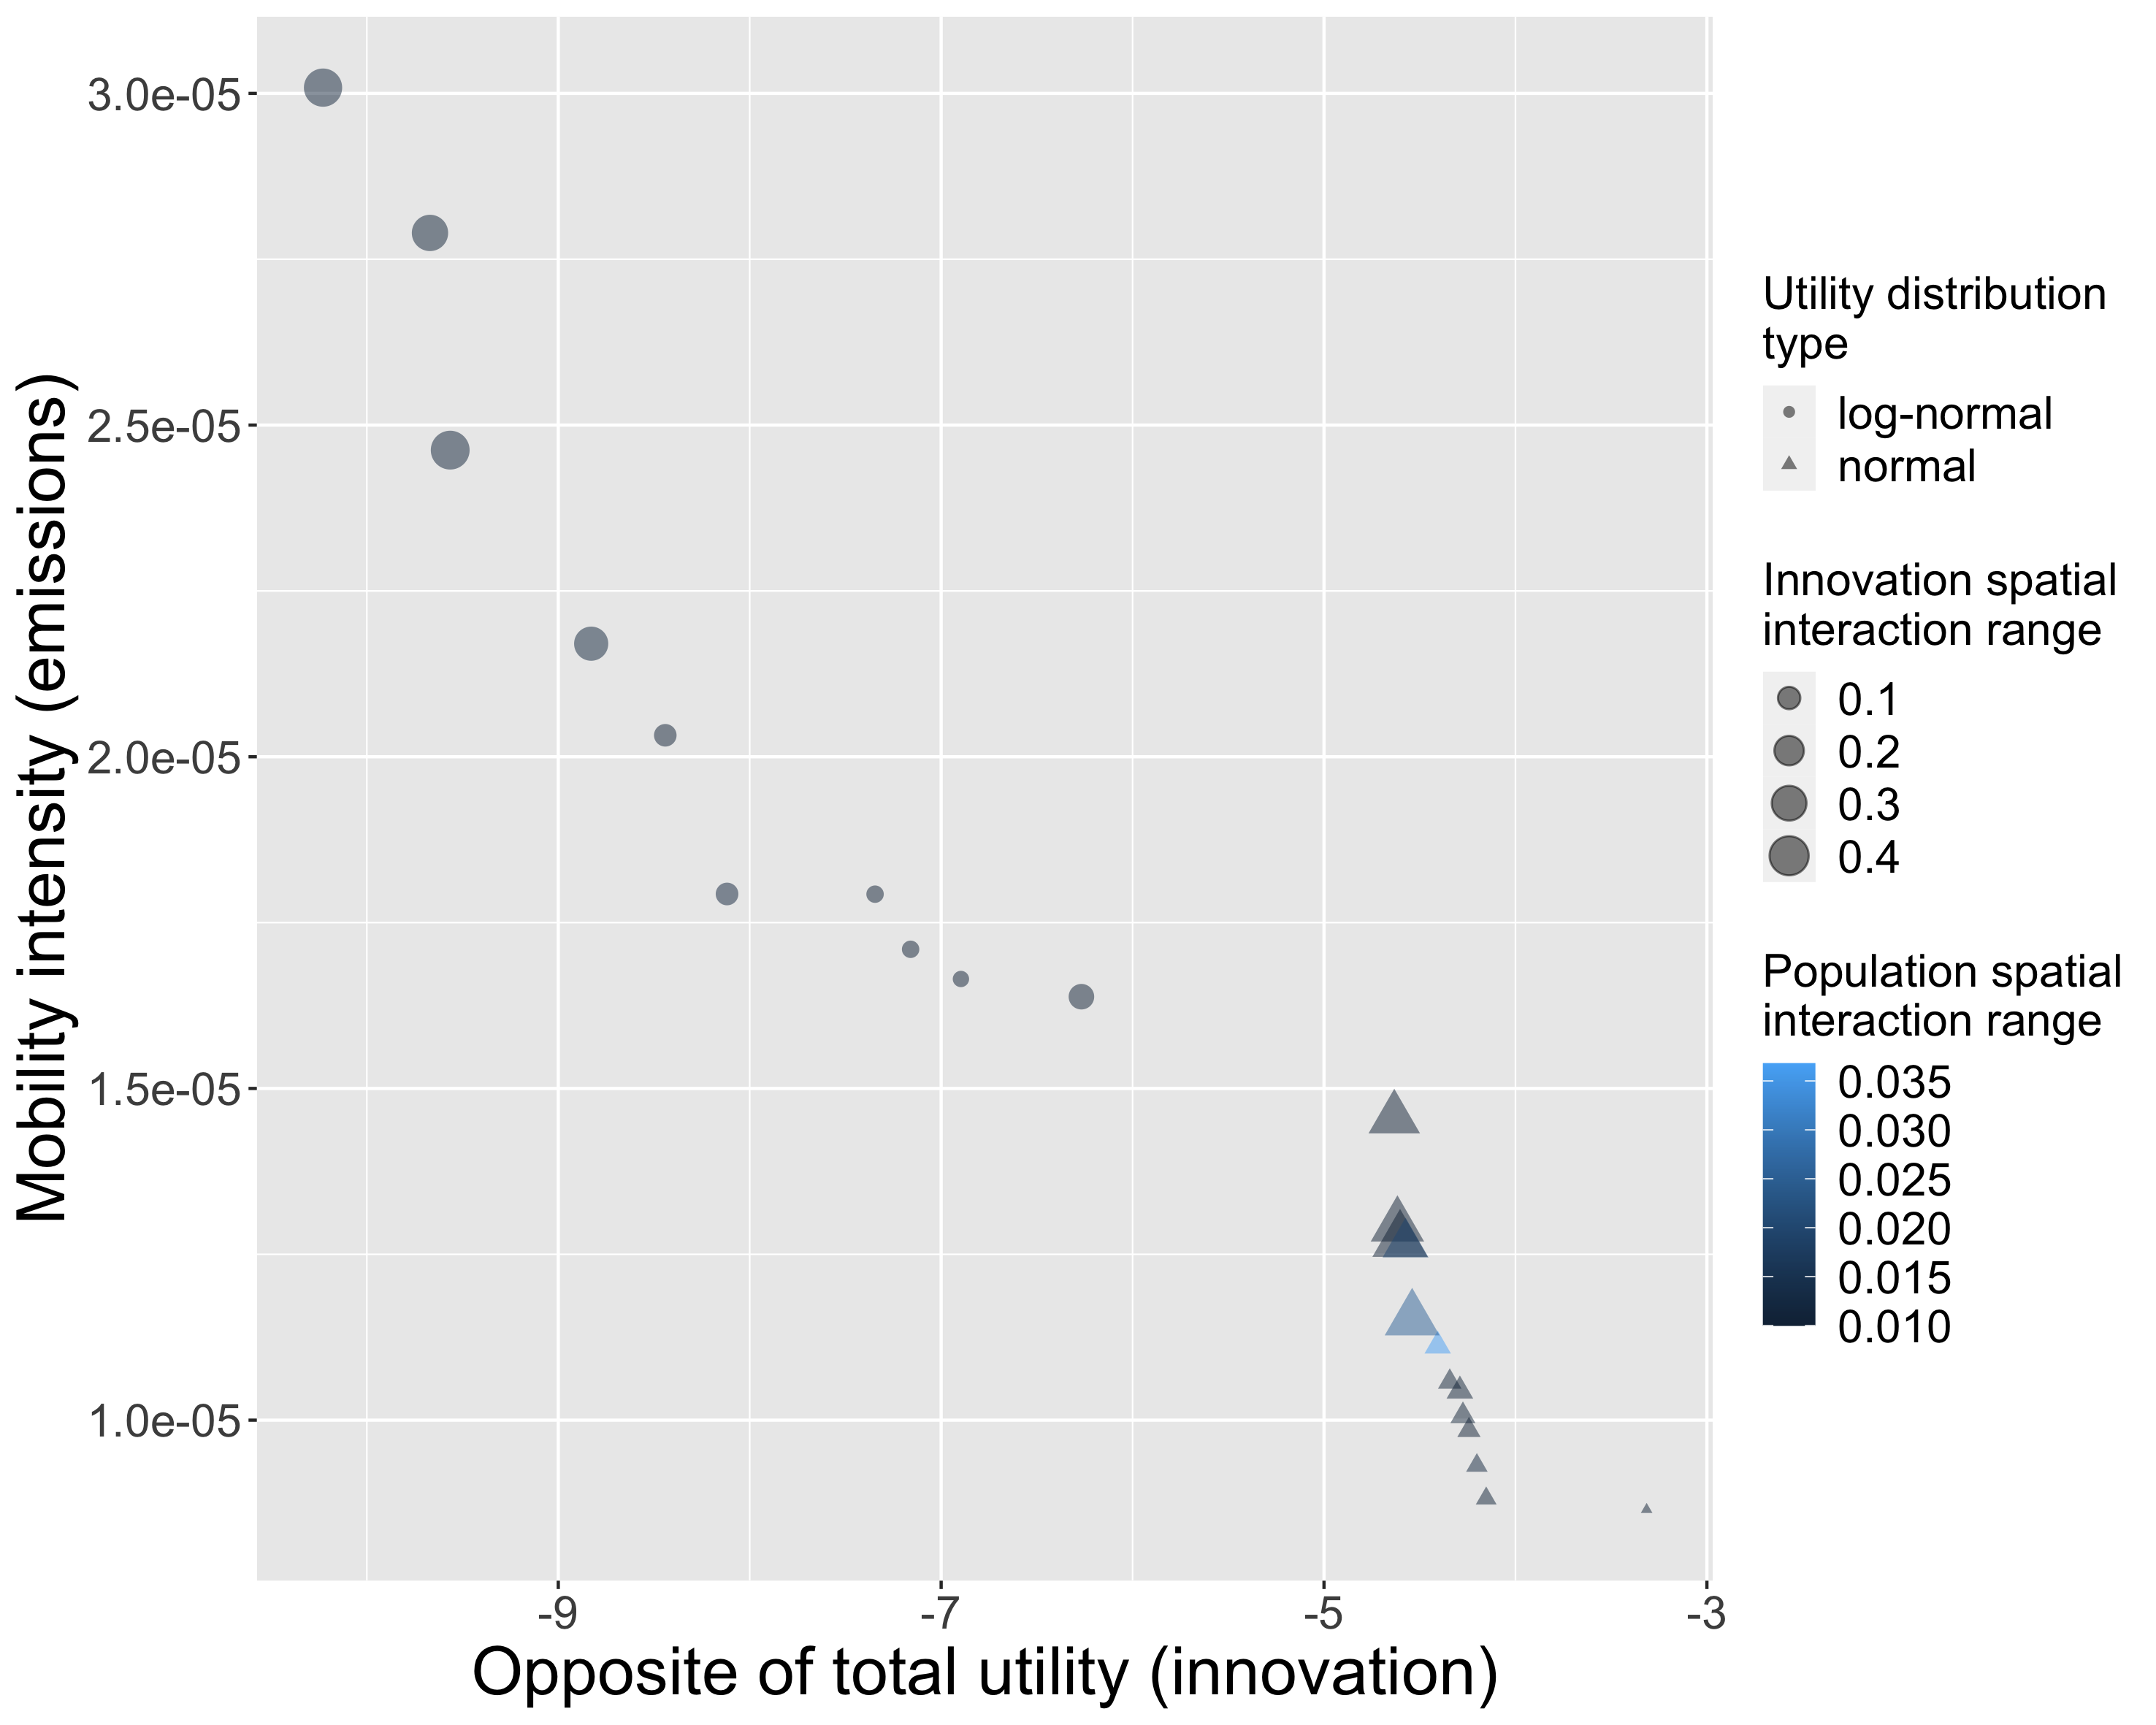
\includegraphics[width=\linewidth]{figures/Fig1.png}
	\caption{Pareto front between the opposite of average utility (innovation) and mobility intensity index (emissions). Point color gives population spatial interaction range; point size innovation diffusion range; and point shape the utility distribution.\label{fig:fig1}}
\end{figure*}

We show optimisation results, as the final algorithm population, in Fig.~\ref{fig:fig1}. We indeed find a broad Pareto front, confirming the existence of a trade-off in such urban dynamics driven by innovation diffusion. We note two parts of the Pareto front, with fat-tailed distributions for utility distribution (log-normal) giving the upper part of the front corresponding to situations with a higher utility but which are more emission intensive. Within this subfront, population spatial interaction are rather local, while a more local innovation diffusion yields less emitting configurations. A similar aspect is observed for the normal distribution subfront, with a U-shaped value of population spatial interactions when going through the front: a more integrated system in terms of population migration produces by itself an intermediate compromise.






\subsection{Conditional optimisation}

% other experiments: conditional to initial hierarchy? innovation hierarchy? -> both useful for policies -> compare Pareto fronts
% Q: normalise by total pop?



\begin{figure*}
	\centering
	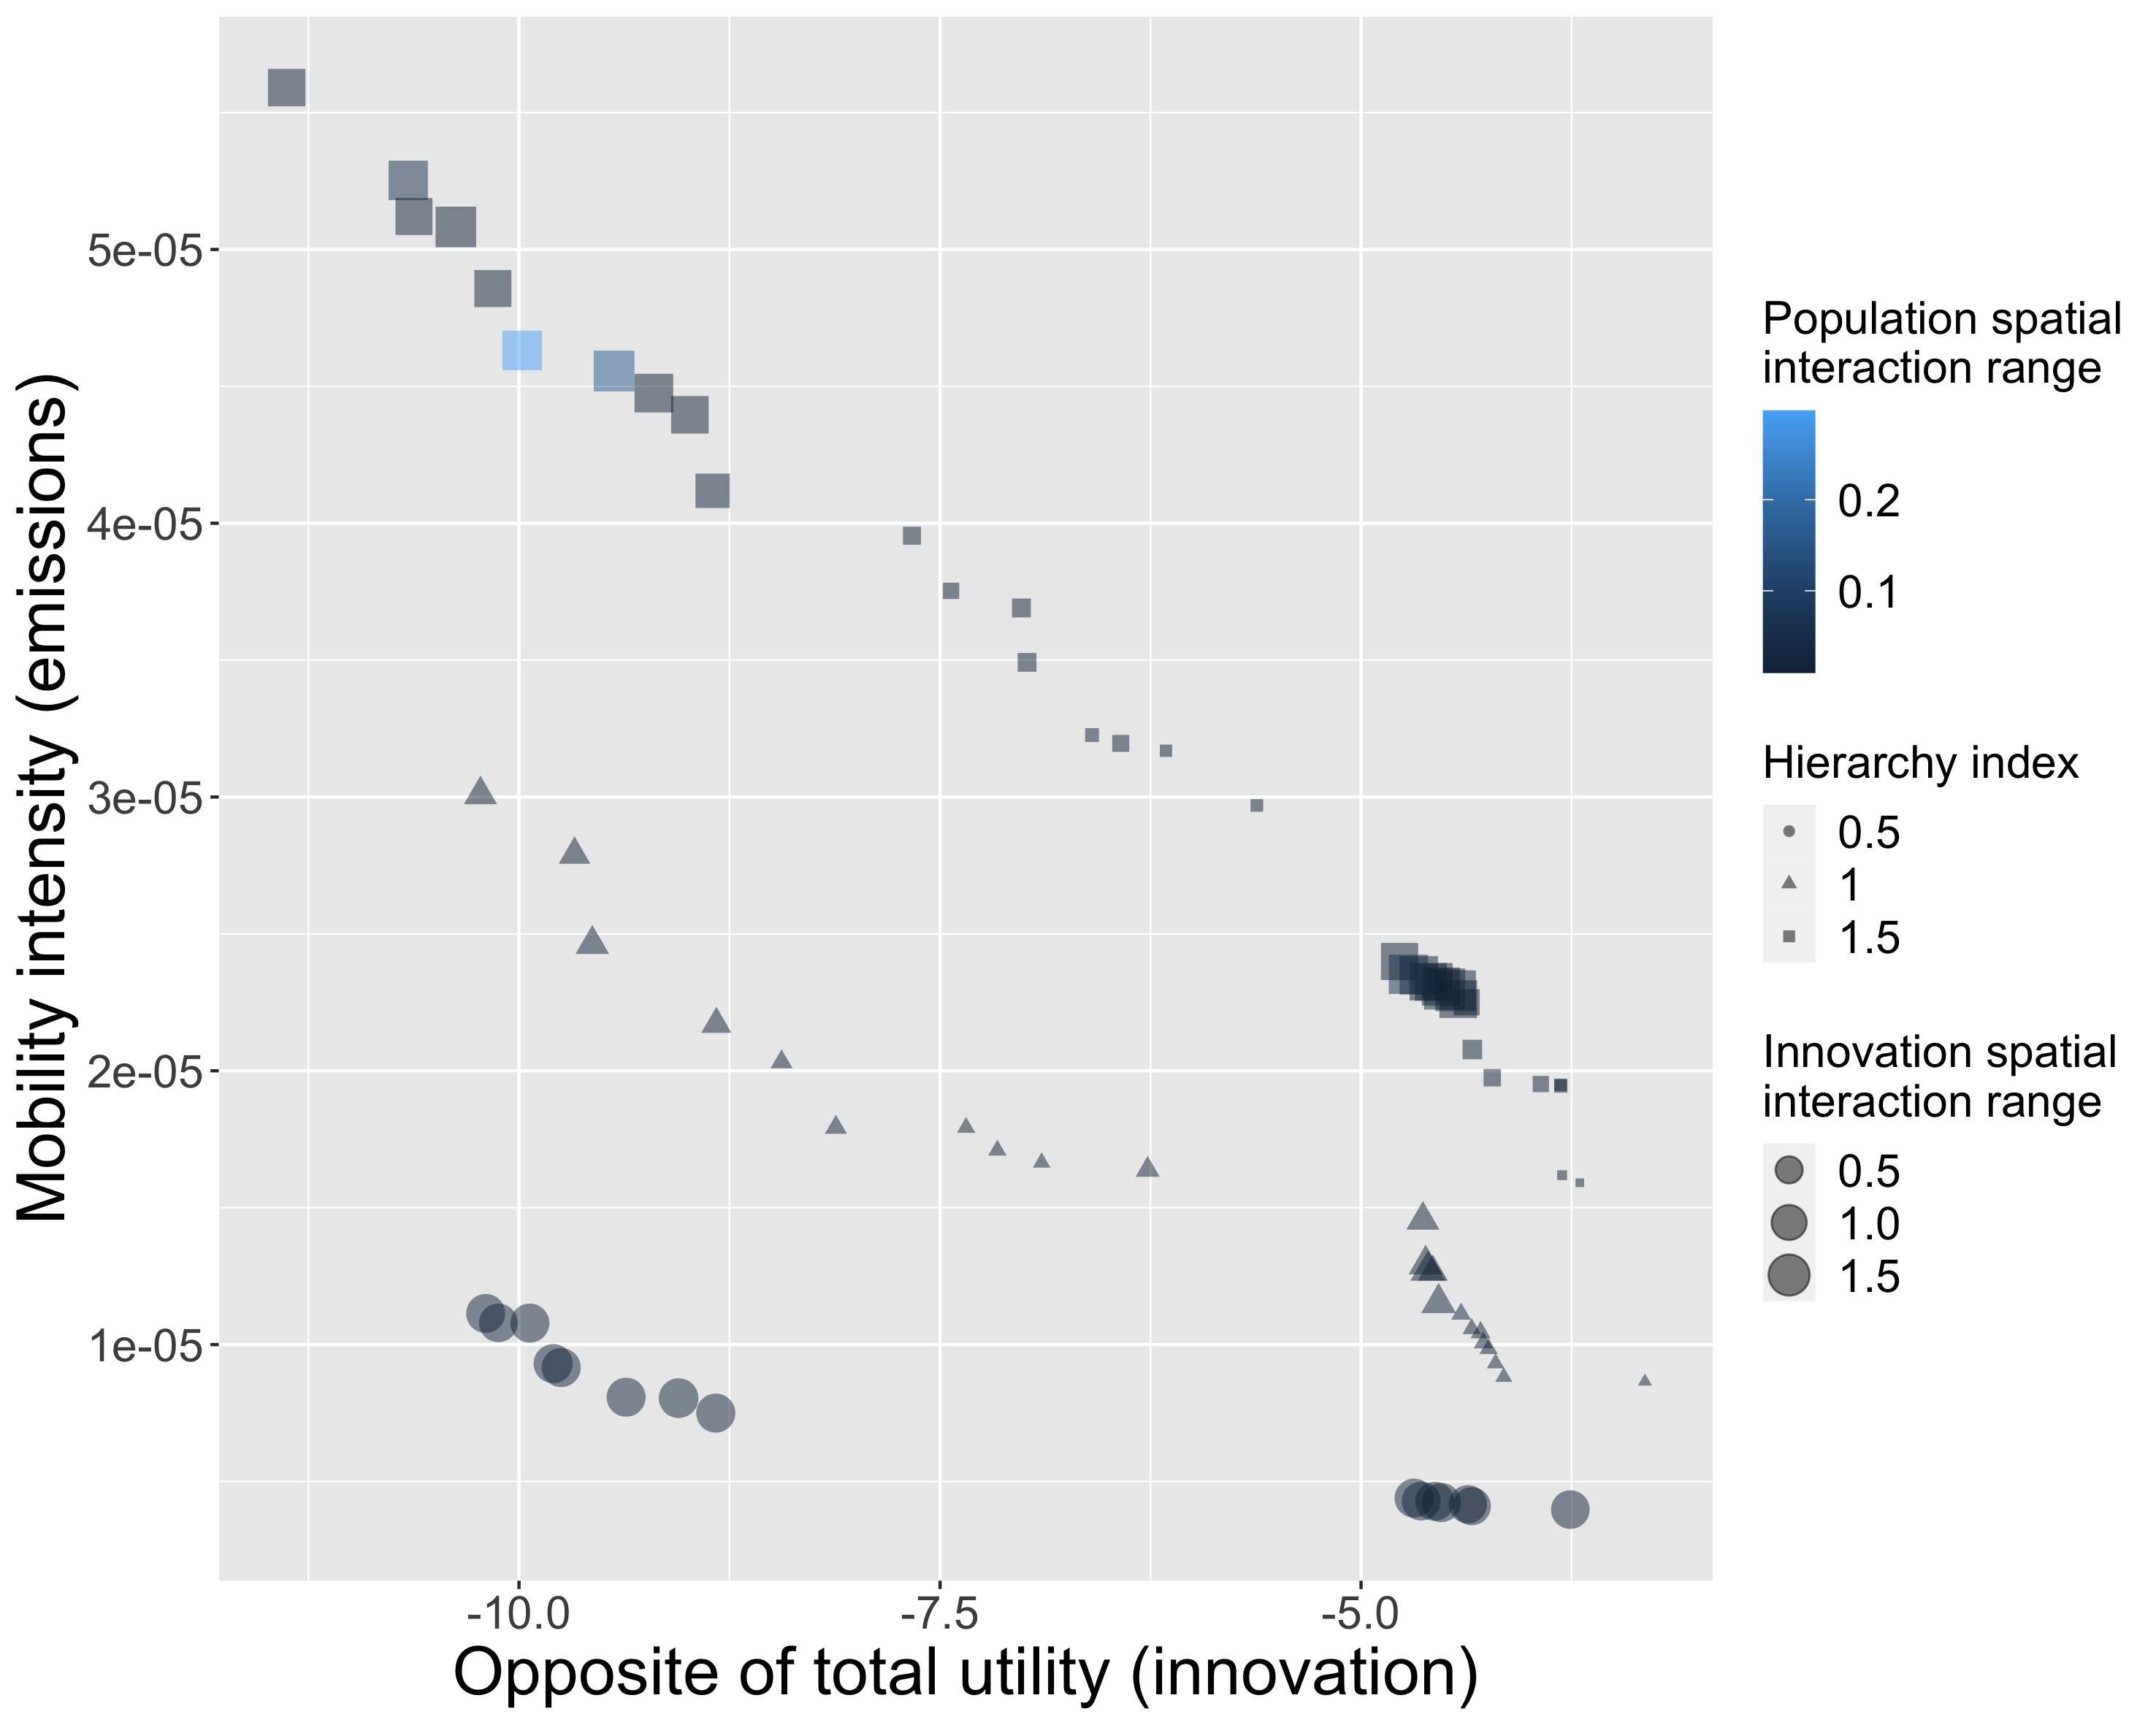
\includegraphics[width=\linewidth]{figures/Fig2.png}
	\caption{Pareto fronts, with initial population hierarchy index fixed at different values (point shape).\label{fig:fig2}}
\end{figure*}


We now turn to experiments which could potentially provide policy insights. We run the same optimisation as before, but changing the initial population hierarchy of cities. To put it simply, we investigate how trade-offs change in different hypothetical systems of cities, ranging from highly hierarchical (Zipf exponent of 1.5) to a more balanced system (exponent of 0.5). We expect to obtain different Pareto fronts, for different values of a hierarchy index, which corresponds to the slope of the initial Zipf law.

We show results in Fig.~\ref{fig:fig2}. We find that the higher the hierarchical inequalities, the less flat the front. Overall, the less hierarchical system dominates the others (but this comparison remains limited as total population is different across systems). Furthermore, the size of the front is the smallest with the less unequal hierarchy, meaning that this system is indeed closer to some global optimum.




\begin{figure*}
	\centering
	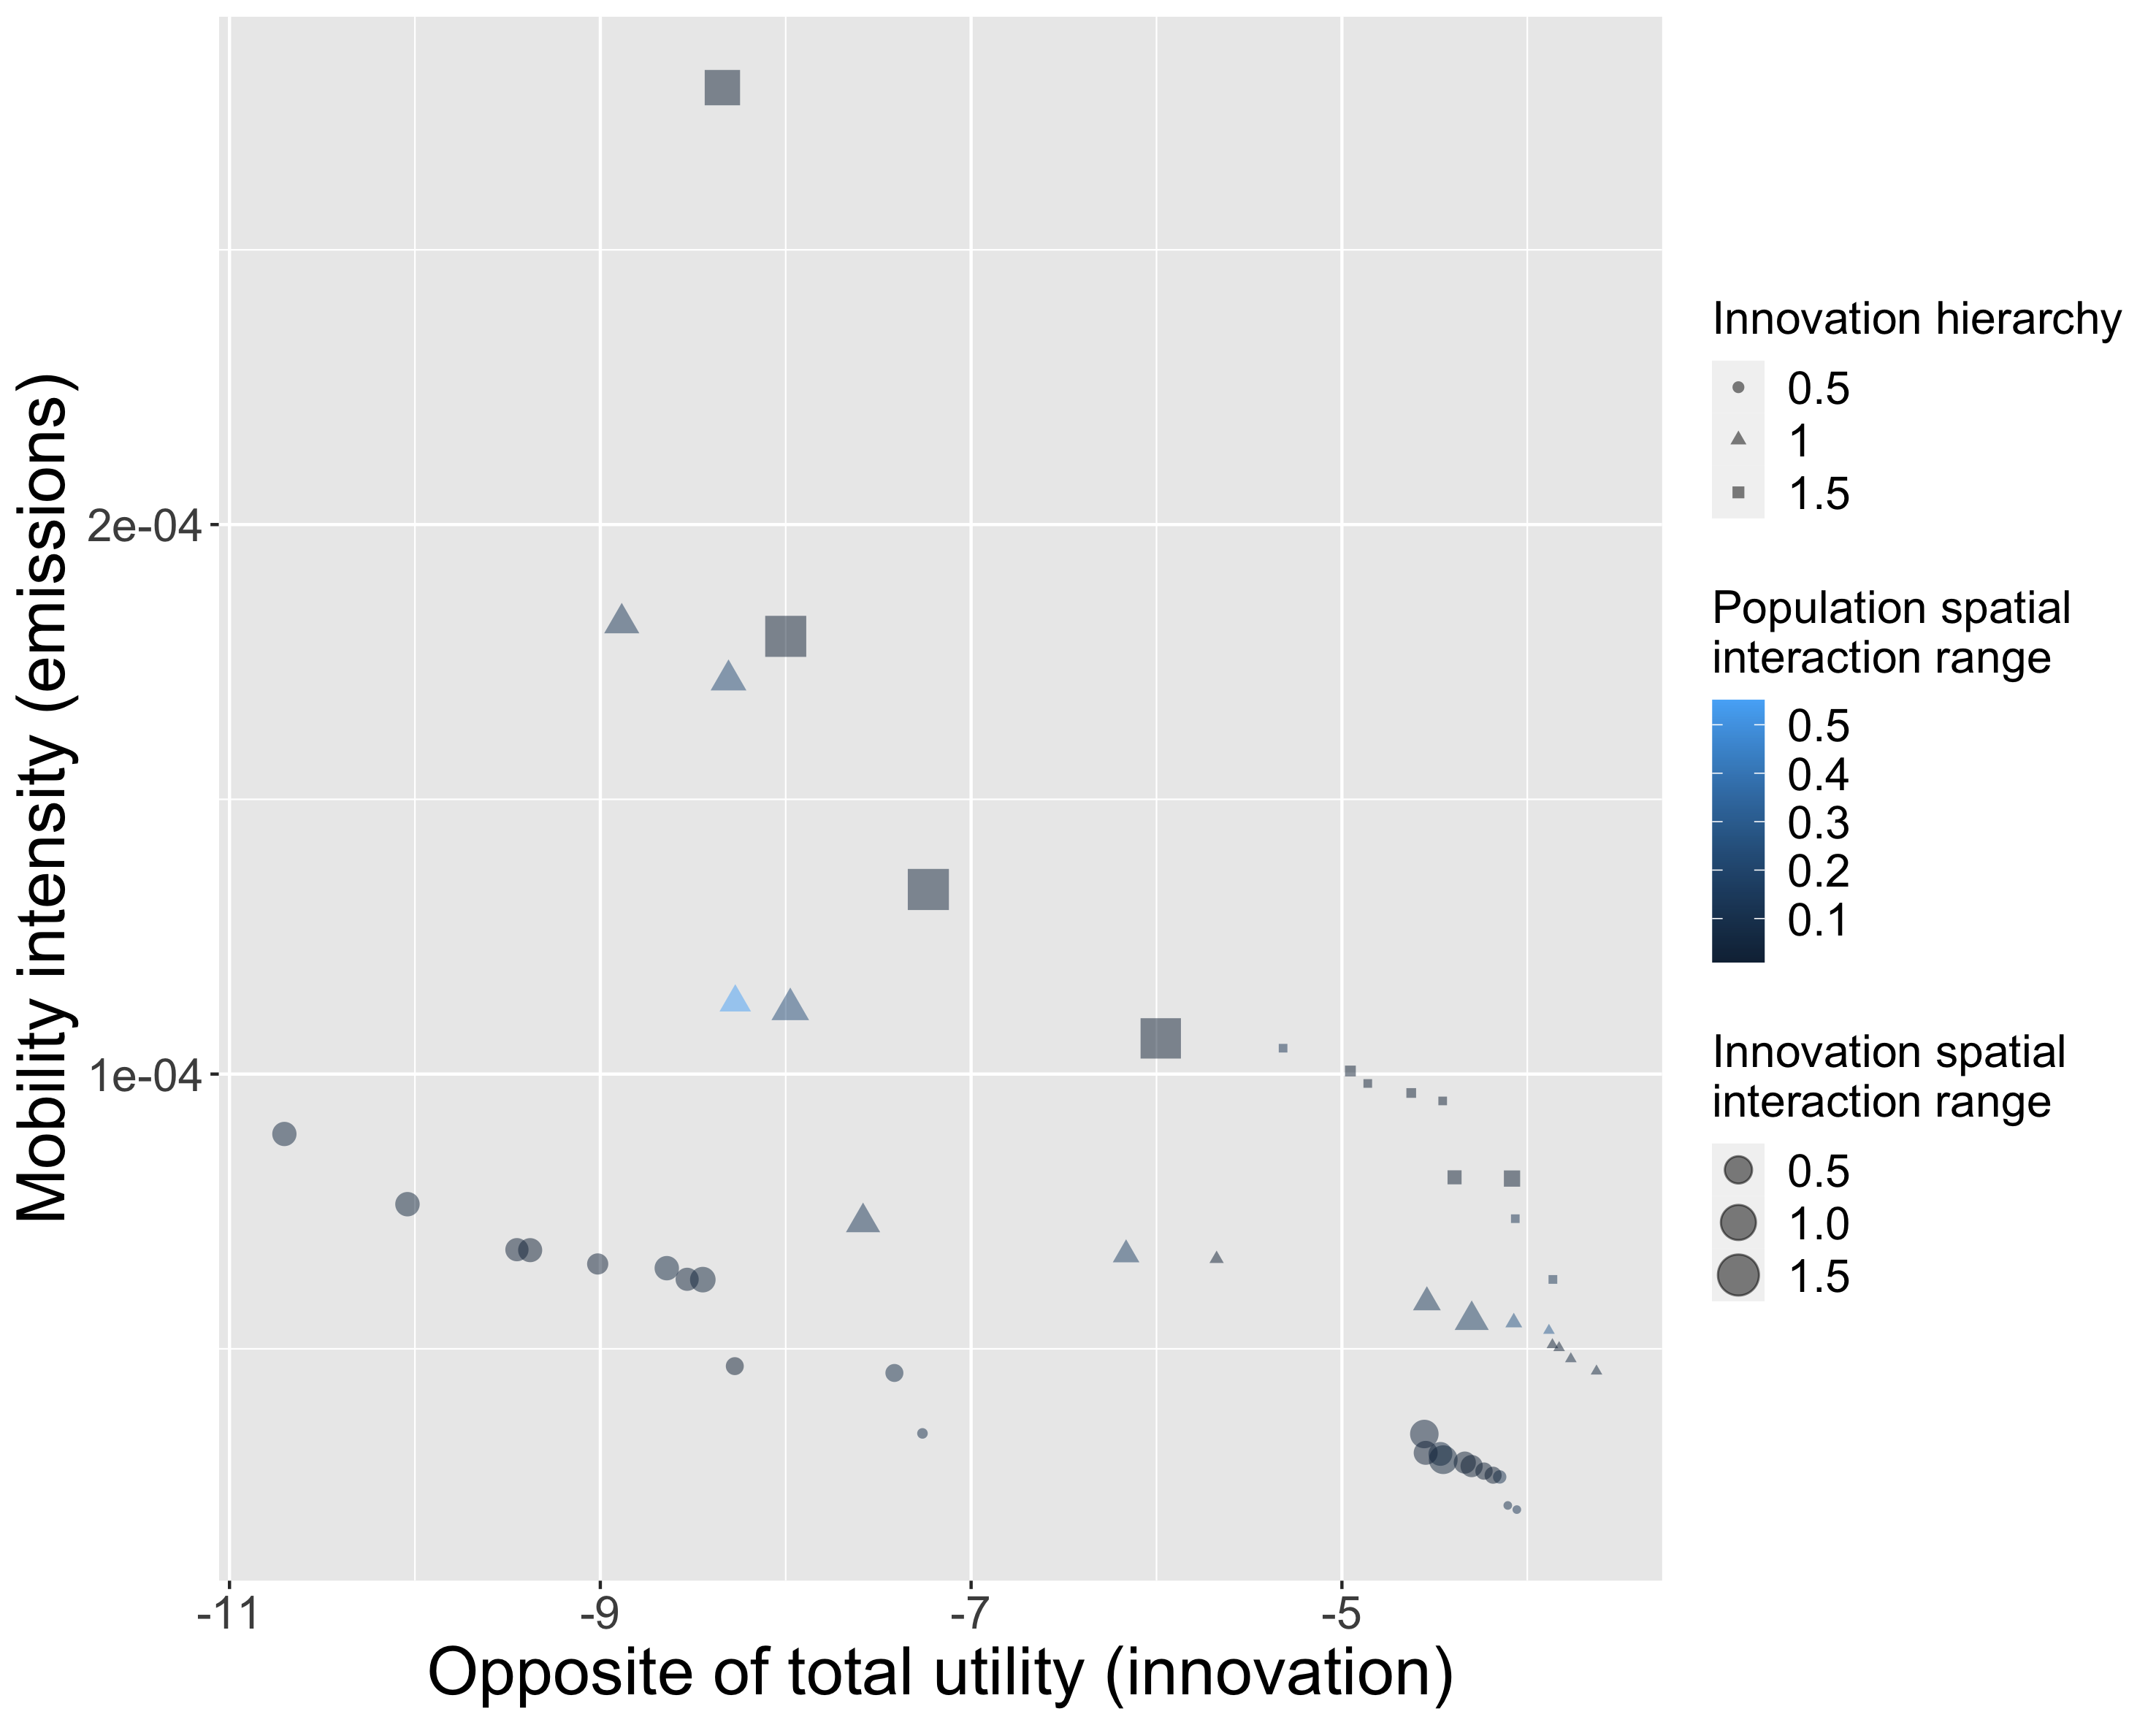
\includegraphics[width=\linewidth]{figures/Fig3.png}
	\caption{Pareto fronts, with innovation hierarchy fixed at different values (point shape).\label{fig:fig3}}
\end{figure*}

We finally show in Fig.~\ref{fig:fig3} a similar conditional optimisation, run by changing the fixed value of innovation hierarchy. This corresponds in terms of policies, to either letting innovation aggregate into larger metropolises (scaling with a high exponent value \cite{pumain2006evolutionary}), or regulating and providing incentives to enhance innovation into smaller and medium-sized cities. We also find that balanced policies provides a more optimal front (they can be compared in this case). Furthermore, this lowest hierarchy corresponds to much higher absolute values of total utility, going against the narrative of a higher value innovation produced by large cities only. Points for the two other fronts are rather close, corresponding to a lower sensitivity when the scaling exponent is larger than one.




\section{Discussion}

We have shown, in a stylised model of urban population and innovation dynamics, that trade-offs between transport emissions and total innovation utility emerge from model dynamics. This has theoretical implications, confirming the general non-optimising nature of urban systems and the predominance of trade-offs across different urban dimensions. Our results from conditional optimisation suggest that less hierarchical systems, both regarding initial population hierarchy and innovation hierarchy, provide more optimal Pareto fronts. This could have implications for policies such as innovation incentives, to avoid a too strong concentration into larger cities. More empirical investigations remain however needed.

Extending this theoretical and stylised work towards more empirical and data-grounded applications raises several issues. First, how to quantify spatial proxies for innovation, to either parametrise the initial configuration, or to calibrate model trajectories in terms of innovation diffusion, remains a difficult question. The use of patent data provides such insights \cite{griliches200713}, but the lack of harmonised and spatialised open patent database limits this perspective. Some initiatives are currently working towards this goal, such as \cite{bergeaud2021patentcity}. Furthermore, more realistic indicators for emissions, both transport and endogenous ones, would be also needed, for example by estimating them through a link with existing emissions databases such as EDGAR \cite{olivier1994emission}.

Adding supplementary optimisation dimensions, to include further SDGs in simulated dynamics, is also an important future model development.
% additional dimensions? wage inequalities \cite{shutters2022urbanization}

Finally, several model limitations would require investigation.

To conclude, we have provided a first stylised insight into trade-offs between SDGs in systems of cities at the macroscopic scale, which can be applied from a theoretical viewpoint to validate or invalidate urban theories, and be used as a basis towards more practical application towards sustainable long-term territorial policies \citep{rozenblat2018conclusion}.



% on kuznet debate: invest in what is working now \cite{brisbois2022climate}



\bibliographystyle{elsarticle-harv} 
\bibliography{biblio}



%% The Appendices part is started with the command \appendix;
%% appendix sections are then done as normal sections
%% \appendix

%% \section{}
%% \label{}


\end{document}

\endinput
